\section{\'Etat de l'art des arbres d'attaques et de défenses}

    \subsection{Théorie des arbres d'attaque et de défense}
        Le concept des arbres d'attaques a été créé en 1999 par Bruce Schneier, un expert américain en securité informatique qui est parti du constat que des systèmes réputés "inviolables" se font briser en permance. De plus, ces systèmes sont brisés non pas en passant au travers des défenses mises en place, mais par des méthodes d'accès qui n'avaient pas été imaginées par ses concepteurs, car ils n'avaient pas les outils pour dresser une liste exhaustive des manières d'attaquer leur système. Il a donc créé le concept des arbres d'attaque dans ce but : pouvoir réaliser un inventaire exhaustif des méthodes d'attaque sur un système, quel qu'il soit, afin de pouvoir en concevoir la défense de la manière la plus complète possible.

<<<<<<< HEAD
	\subsection{Théorie des arbres d'attaques et de défenses}
		Le concept des arbres d'attaques a été introduit en 1999 par Bruce Schneier, un expert américain en securité informatique qui est parti du constat que des systèmes réputés "inviolables" se font briser en permance. De plus, ces systèmes sont brisés non pas en passant au travers des défenses mises en place, mais par des méthodes d'accès qui n'avaient pas été imaginées par ses concepteurs, car ils n'avaient pas les outils pour dresser une liste exhaustive des manières d'attaquer leur système. Il a donc imaginé le concept des arbres d'attaque dans ce but : pouvoir réaliser un inventaire exhaustif des méthodes d'attaque sur un système, quel qu'il soit, afin de pouvoir en concevoir la défense de la manière la plus complète possible. Schneier a lui-même imaginé son modèle d'arbre d'attaque à partir du concept des "Arbres de Défaillances", une méthodologie datant du début des années soixante dont le but est de pouvoir évaluer l'impact de la défaillance d'un composant sur le système dont il fait parti. 

		Lors de ces recherches, Schneier a retenu un formalisme prècis : Une représentation des menaces sous la forme d'arbres. Ces arbres sont réalisés en se posant la question suivant : Si je veux atteindre tel objectif, qu'est ce que cela pré-suppose que j'accomplisse d'abord ? Pour cela, on représente l'objectif final à la racine de l'arbre (en haut), et l'on ajoute en descendant dans l'arbre des Noeuds représentant des objectifs intermédiaires à réaliser et qui nous garantissent l'accomplissement de l'objectif principal. L'ajout de ces noeuds peut se faire sous deux formes distinctes : par disjonction ou conjonction. La disjonction correspond à des cas où un seul des noeuds inférieurs valide le noeud supérieur (opération logiquie OU, représentée par des traits simples). La conjonction quant-à elle correspond à des cas où il faut valider l'ensemble des noeuds inférieurs pour valider le noeud supérieur (opération logiquie ET, représentée par des traits simples reliés entre eux par un arc). L'on fait ensuite découler de ces objectifs intermédiaires d'autres objectifs les validant et ainsi de suite, jusqu'à avoir les actions de base aux feuilles de l'arbre (en bas). Ensuite, il suffit de descendre dans l'arbre à partir d'un noeud pour savoir quelles sont les combinaisons d'actions possibles à effectuer pour atteindre le noeud. Les éléments (noeuds et feuilles) sont traditionnellement représentés par des ronds.

		Enfin, le modèle des arbres d'attaques intègre la possibilité d'associer aux feuilles des valeurs représentatives de diverses informations sur l'accomplissement de l'action : coût, difficulté, probabilité, temps d'exécution, etc... Ces valeurs permettent alors de quantifier le "poids" du noeud dans l'arbre vis-à-vis de l'attaquant.  Il est alors possible à partir de ces valeurs de pouvoir quantifier ces mêmes informations pour les noeuds qui en découlent (par exemple, le poids d'un noeud OU peut avoir le poids minimal parmi ces noeuds inférieurs, tandis que dans le cas d'un noeud ET son poids sera leur somme), ce qui peut servir à l'attaquant pour choisir une stratègie d'attaque plutôt qu'une autre au vu de ses ressources.

		L'arbre de la Figure \ref{fig:arbre_exemple_1} illustre ce formalisme : 

		\begin{figure}
			\begin{center}
				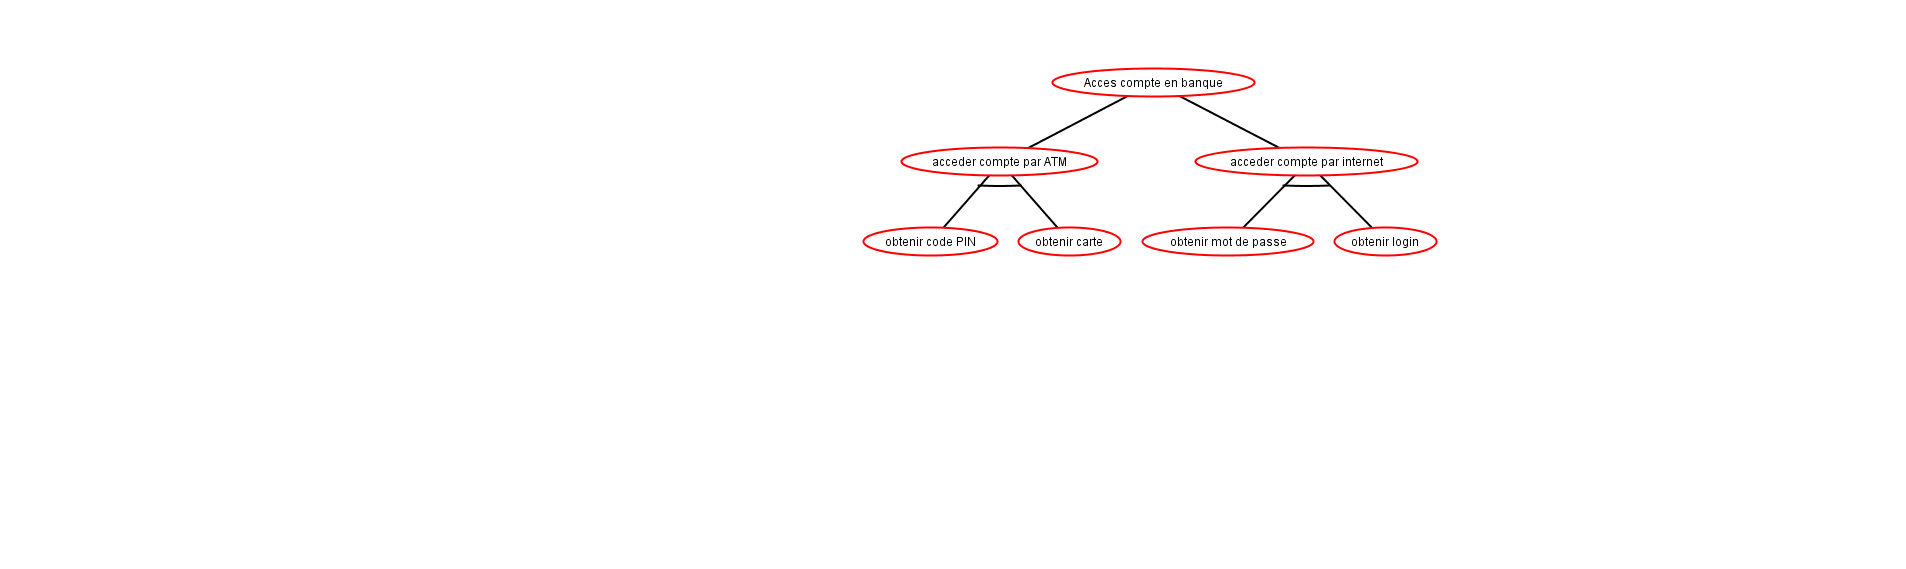
\includegraphics[width=0.8\textwidth]{figure/exemple1_rapport.png}
			\end{center}
			\caption{Exemple d'arbre d'attaques}
			\label{fig:arbre_exemple_1}
		\end{figure}

		Depuis 1999, le concept a évolué grâce à la contribution de personnes ayant étendu et amélioré le concept de Schneier. Ces personnes ont en particulier étendu le concept d'arbre d'attaque à celui d'arbre d'attaques et de défenses, aussi appelé Attack-Defense-Tree (ADTree), où sont également représentés les defenses mises en place et que le potentiel attaquant aura besoin de désactiver pour atteindre son but. Les défenses sont traditionnellement représentés par des rectangles. Le même cas que précédemment pour lequel des défense auraient été mises en place pourrait correspondre à la Figure \ref{fig:arbre_exemple_2}.

        \begin{figure}[h!]
            \begin{center}
                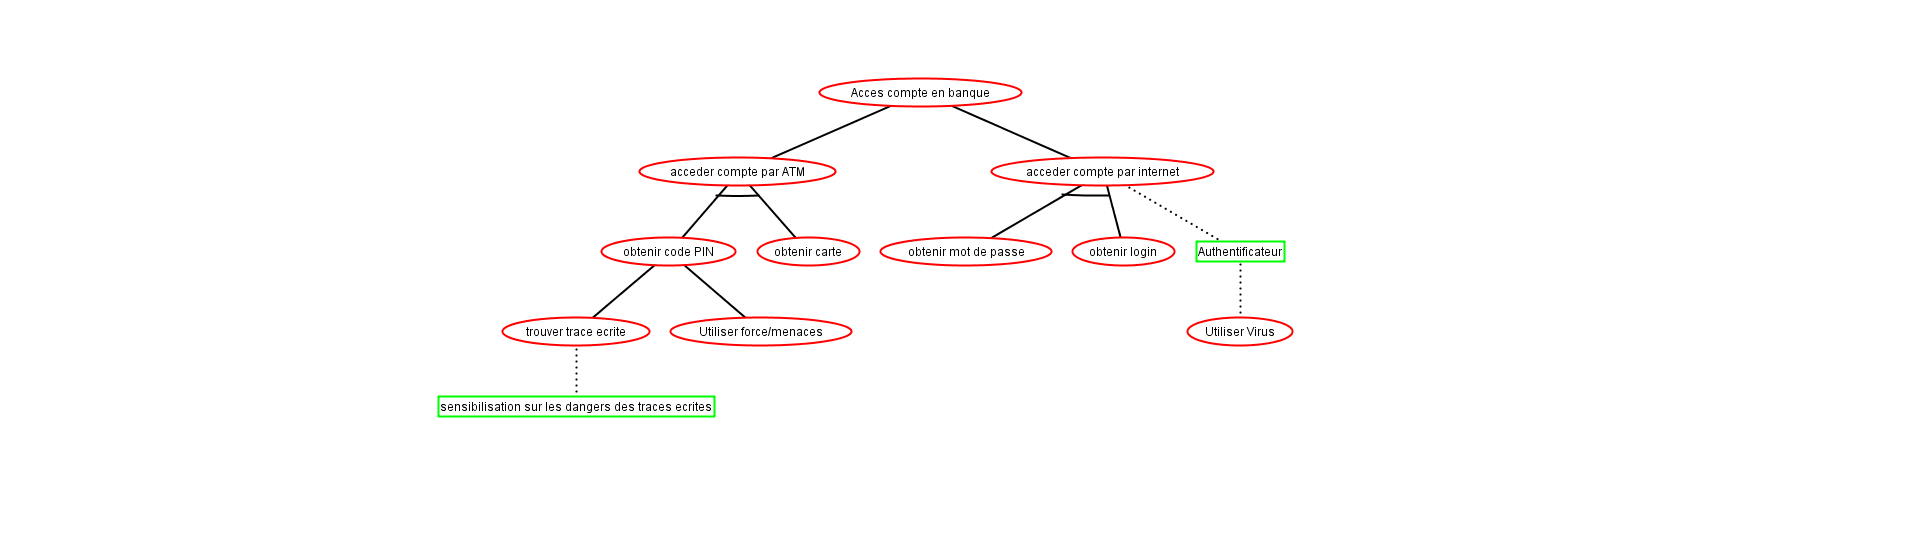
\includegraphics[width=1\textwidth]{figure/exemple2_rapport.png}
            \end{center}
            \caption{ADTree}
            \label{fig:arbre_exemple_2}
        \end{figure}

<<<<<<< HEAD
	\section{Implémentations des ADTree}
		Plusieurs logiciels implémentant le concept des arbres d'attaques ou des ADTree ont été développés. Exemples :
        
        {\large Logiciels propriétaires :}
        \begin{itemize}
            \item SecurlTree : logiciel de création et d'analyse d'arbres d'attaques développé par la société Amenaza
            \item ATTACKTREE+ : logiciel de création et d'analyse d'arbres d'attaques développé par la société Isograph
        \end{itemize}
        ~~\\
        {\large Logiciels Open-Source :}
        \begin{itemize}
            \item ADTool : Logiciel développé par une équipe de chercheur de l'université du Luxembourg pour la modélisation d'ADTrees (le logiciel avec lequel nous allons travailler)
        \end{itemize}
~~

        Aujourd'hui, les arbres d'attaques tels qu'introduits par Schneier sont utilisés par de nombreuses entreprises. Ceci est dû à l'avantage de pouvoir partir du point de vu de l'attaquant et donc de concentrer les efforts de défenses là où ils seront le plus utiles, à l'inverses d'un certain nombres d'autres stratègies de défense qui vont se concentrer seulement sur la défense du point de vue du défenseur (par exemple les arbres de défaillance), aboutissant forcement à une estimation des dangers incomplète. 

        Cela dit, un grand nombre de ces entreprises développent en interne leur propre logiciel de construction et d'analyse des arbres d'attaque/défense sans toutefois utiliser ceux présent sur le marché. En effet, les solutions logicielles ne bénéficient pas d'une grande visibilité, peuvent être chères et ne sont pas forcement faciles à mettre en place. De plus, le nombre de logiciels implémentant les ADTree est assez réduit en comparaison de ceux implémentant les arbres d'attaques. Ceci étant, le développement peut être laborieux même en utilisant un logiciel dédié comme ADTool pour plusieurs raisons : le logiciel n'intégre pas d'arbres génériques ce qui ralonge le développement et oblige de modéliser plusieurs fois la même partie d'arbre, ne permet pas non plus de gérer la quantification de manière dynamique selon qui est l'attaquant, etc.

        Un grand nombre d'amélioration est donc possible : Ce qui nous amène au cahier des charges.

        % Biblio :
        % https://www.schneier.com/paper-attacktrees-ddj-ft.html
        % http://www.sciencedirect.com/science/article/pii/S1574013714000100
        % http://logcom.oxfordjournals.org/content/24/1/55
        % http://www.infres.enst.fr/people/leneutre/SECUR/INF941-Intro-securite-2011-12.pdf
        % http://www.labunix.uqam.ca/~gingras_e/Inf4470/Pres_Vulnerabilites.pdf
        % http://tel.archives-ouvertes.fr/docs/00/46/25/34/PDF/these-eric_lacombe.pdf

